\documentclass[12pt,a4paper,openright,twoside]{book}
\usepackage[utf8]{inputenc}
\usepackage{disi-thesis}
\usepackage{code-lstlistings}
\usepackage{notes}
\usepackage{shortcuts}
\usepackage{acronym}
\usepackage[acronym]{glossaries}
\usepackage{float}

\school{\unibo}
\programme{Corso di Laurea Triennale in Ingegneria e Scienze Informatiche}
\title{Uso del Machine Learning per la detection dei domini DGA \break (Domain Generation Algorithm)}
\author{Simone Collorà}
\date{\today}
\subject{Programmazione a Oggetti}
\supervisor{Prof. Mirko Viroli}
%\cosupervisor{Dott. Gianluca Aguzzi}
%\morecosupervisor{Dott. CoSupervisor 2}
\session{I}
\academicyear{2024-2025}

% Definition of acronyms
\acrodef{IoT}{Internet of Thing}
\acrodef{vm}[VM]{Virtual Machine}
\newacronym{DGA}{DGA}{Domain Generation Algorithm}
\newacronym{C&C}{C\&C}{Command and Control}
\newacronym{P2P}{P2P}{Peer to Peer}
\newacronym{IRC}{IRC}{Internet Relay Chat}


\mainlinespacing{1.05} % line spacing in mainmatter, comment to default (1) before it was 1.241

\begin{document}
\frontmatter\frontispiece
\nocite{*}

\begin{abstract}	
Max 2000 characters, strict.
\end{abstract}



%----------------------------------------------------------------------------------------
\tableofcontents   
\listoffigures     % (optional) comment if empty
%\lstlistoflistings  (optional) comment if empty
%----------------------------------------------------------------------------------------

\mainmatter

%----------------------------------------------------------------------------------------
\chapter{Introduzione}
\label{chap:introduction}
%----------------------------------------------------------------------------------------

La sicurezza informatica è un argomento di crescente importanza
nel mondo moderno. Con il passare del tempo,
i sistemi di protezione sono diventati sempre più sofisticati
e potenti ma, allo stesso tempo, anche gli hackers 
hanno sviluppato tecniche sempre più avanzate per eludere i sistemi di protezione.
Tra queste vi è sicuramente l'uso di Botnets
dei \acrfull{C&C} servers. I \acrshort{C&C} sono dei server che manipolano
i computer infetti da malwares, i Botnets, permettendo
all'attaccante di eseguire codice malevolo da remoto.
Il malware, però, deve conoscere un indirizzo IP o un dominio
per contattare il server. L'attaccante potrebbe
inserire in modo bruto l'indirizzo IP del server nel codice del malware,
ma questo metodo è facilmente rilevabile e bloccabile.
Gli hackers, quindi, preferiscono utilizzare dei domini
generati in modo pseudo casuale per nascondere i loro server chiamati
\acrfull{DGA} servers. Negli ultimi anni, sono stati sviluppati
vari metodi di Machine Learning per rilevare questi domini.



\paragraph{Struttura della tesi}
Il lavoro di tesi si dividerà in 4 capitoli. Nel primo
capitolo verrano descritti concetti di base riguardanti \acrshort{DGA} e Botnets,
e Machine Learning con una breve descrizione delle reti neurali e di alcuni
algoritmi usati. Nel secondo capitolo verrà descritto il progetto,
i suoi obiettivi e i risultati ottenuti. Nell'ultimo capitolo
verranno discusse le conclusioni e i possibili sviluppi futuri.

%\note{At the end, describe the structure of the paper}

\chapter{Background}

Di seguito sono descritti i concetti base su cui si basa il progetto.

\section{Domain Name System}
Il \textbf{Domain Name System} (DNS) è un sistema che
traduce un nome di dominio in un indirizzo IP.



\section{Botnets e DGA}

\subsection{Botnets}

I Botnets sono reti di computer infetti da malware, chiamati bot,
che possono essere controllati da un attaccante, il botmaster.
La vita di un botnet nella maggior parte dei casi è divisa in 4 fasi:
\begin{enumerate}
    \item \textbf{Infezione e propagazione}: Questo è il primo
    passaggio. L'attaccante cerca di infettare un computer
    tramite vari metodi come email con link malevoli o \acrfull{P2P} sharing.
    Una volta infettato un dispositivo, il malware cerca di infettare
    altri dispositivi nella rete.

    \item \textbf{Rallying}: i bots cercano di contattare per la prima volta
    il server \acrshort{C&C} per far capire all'attaccante
    che l'attacco è andato a buon fine.

    \item \textbf{Commands and Reports}: il malware esegue le istruzioni
    ricevute dal server \acrshort{C&C} e invia i risultati al botmaster.
    I bots ascoltano continuamente il server \acrshort{C&C} 
    o si connettono ad esso periodicamente. Appena ricevono
    un comando lo eseguono, inviano i risultati al botmaster
    e aspettano un nuovo comando.

    \item \textbf{Abbandono}: Quando un bot non è più utile o utilizzabile,
    il botmaster può decidere di abbandonarlo. Il botnet, invece,
    sarà completamente distrutto quando tutti i bot saranno
    abbandonati o bloccati dalla vittima o quando il \acrshort{C&C} server
    verrà bloccato


\end{enumerate}

\begin{figure}[H]
    \centering
    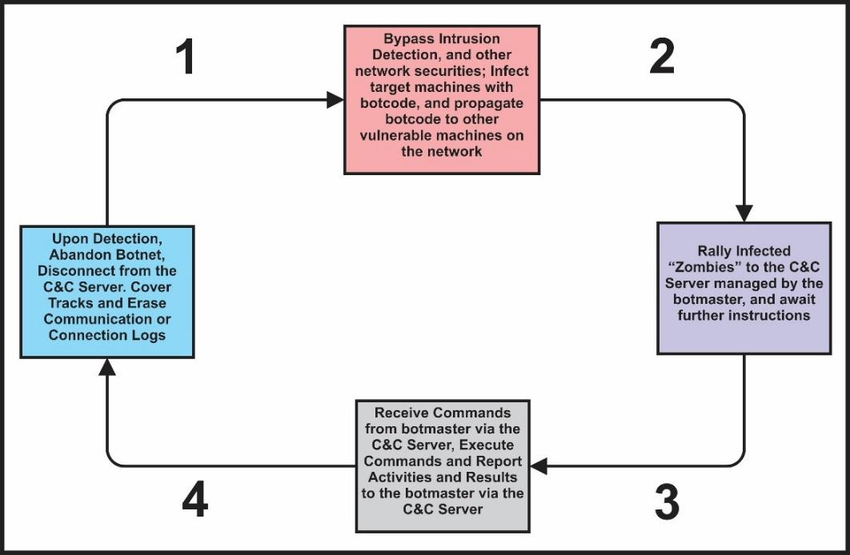
\includegraphics[width=.8\linewidth]{figures/The-Lifecycle-Schema-of-a-typical-Botnet.png}
    \caption{Ciclo di vita di un botnet \cite{Ogu2016}}
    \label{fig:botnet}
\end{figure}

\subsection{Command and Control} 

Il meccanismo del \acrshort{C&C} crea un canale di comunicazione
tra il botmaster e i bot. Questo è essenziale per il funzionamento
del botnet. Ci sono tre tipi di server \acrshort{C&C}:

\begin{itemize}
    \item \textbf{Centralizzati}: In questo tipo di server, il botmaster
    controlla tutti i bot tramite un server centrale. Questo è il metodo
    più semplice e veloce per controllare i bot ma è anche il più vulnerabile.
    Se il server centrale viene bloccato, tutti i bot non possono più
    ricevere comandi. Questo a sua volta è diviso in due categorie:
    \begin{itemize}
        \item \textbf{IRC} : \acrfull{IRC} è un sistema di chat
        usato per comunicare tra i bot e il botmaster in tempo reale.
        Questo era più usato nella prima generazione di botnet. 
        I bot si connettono al server \acrshort{IRC} e aspettano
        i comandi dal botmaster. I bot seguono un approccio PUSH ovvero
        quando un bot si connette ad un determinato canale, esso rimane connesso.
        \item \textbf{HTTP / HTTPS}: Il più usato. Con questa tecnica, i bot usano un URL o IP
        per contatattare il server \acrshort{C&C}. Qua invece i bot seguono
        un approccio PULL. I bot si connettono al server \acrshort{C&C}
        periodicamente e controllano se ci sono nuovi comandi. Questo processo
        va ad intervalli regolari definiti dal botmaster.
    \end{itemize}

    \item \textbf{Decentralizzati}: Questo tipo di \acrshort{C&C}
    è basato su un sistema \acrshort{P2P} senza un server centrale. In questo modo,
    computer infetti fanno sia da bot che da server \acrshort{C&C}.
    Questo metodo è più difficile da rilevare ma anche
    più complesso da implementare \cite{4804459}.

\end{itemize}

\begin{figure}[H]
    \centering
    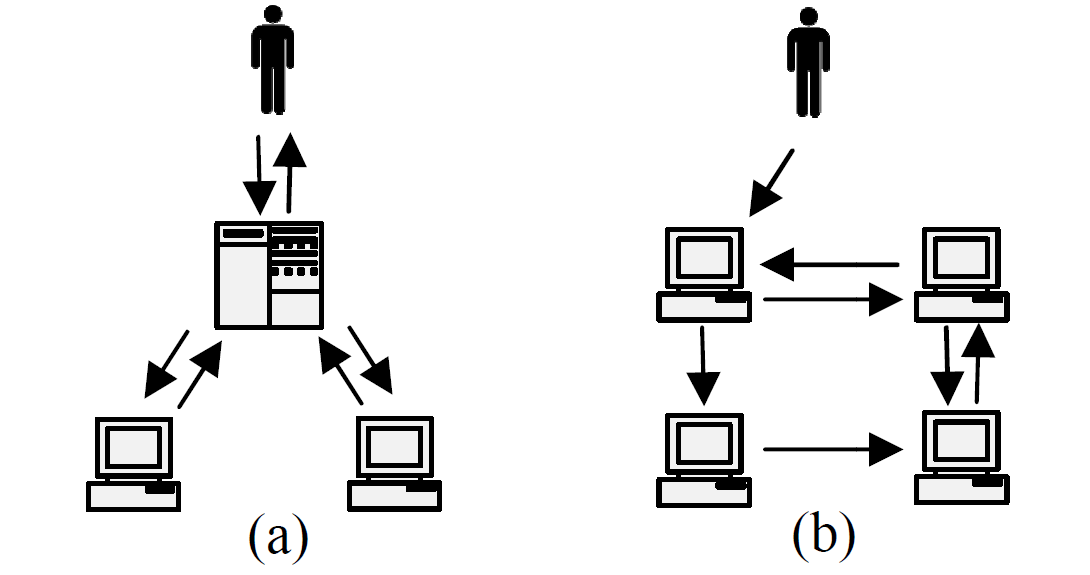
\includegraphics[width=.8\linewidth]{figures/Types-of-CC.png}
    \caption{Esempio di server \acrshort{C&C}. (a) centralizzato, (b) decentralizzato \cite{6487169}}
    \label{fig:command and control}
\end{figure}

\subsection{Domain Generation Algorithm}

I \acrshort{DGA} sono algoritmi che generano migliaia di domini in modo pseudo casuale.
Prima viene scelto un seed, di solito la data odierna
o anche le previsioni meteo \cite{8621875} e, tramite
un algoritmo di hashing, vengono generati i domini.
Questi domini vengono poi utilizzati per contattare i server \acrshort{C&C}.
Non tutti i domini generati però sono registrati.
Il computer infetto, tramite i DNS locali, cercherà di tradurre
un dominio in un indirizzo IP.
Se non riesce a contattarlo con un determinato dominio,
proverà con il successivo finché non troverà
un dominio valido che permetterà al malware di comunicare con
il server \acrshort{C&C} \cite{8489147}.
In questo modo, diventa più difficile per i sistemi di protezione
rilevare e bloccare i loro attacchi.
Si potrebbe pensare di bloccare direttamente i domini tramite
una blacklist ma questo metodo
risulta inefficace poiché vengono generati migliaia di domini
continuamente. Si pensi che Conficker C, un famoso malware
che utilizza \acrshort{DGA}, è in grado di generare
fino a 50.000 domini pseudo casuali al giorno \cite{978131}.
Un altro modo per contrastare ciò
potrebbe essere quello di fare reverse engineering
del \acrshort{DGA} per capire quale seed viene utilizzato per generare i domini.
Questo però risulta lento e dispendioso e possibilmente inefficace \cite{8887881}.

\begin{figure}[H]
    \centering
    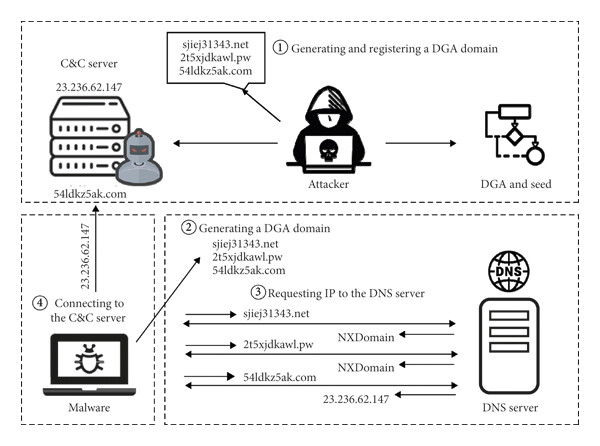
\includegraphics[width=.8\linewidth]{figures/DGA example.jpg}
    \caption{Esempio del funzionamento di un \acrshort{DGA} \cite{8887881}}
    \label{fig:DGA example}
\end{figure}

Per contrastare i \acrshort{DGA}, sono stati sviluppati
vari metodi di Machine Learning in grado di rilevare i domini generati.
Questi metodi hanno due lati poisitivi:
\begin{itemize}
    \item Non richiedono un lungo processo di reverse engineering.
    \item Essendo l'AI una blackbox, è molto difficile
    per gli hackers eseguire un reverse engineering del modello.
\end{itemize}

\section{Machine Learning}
Il Machine Learning è una branca dell'informatica che punta
a far ragionare le macchine come gli esseri umani, ovvero
a svolgere compiti autonomamente senza essere programmati
esplicitamente e migliorando le loro prestazioni con l'esperienza
e i dati.



\subsection{Reti Neurali}

Una \textbf{Rete Neurale} o in inglese \textbf{Artificial Neural Network} (ANN) è
un modello matematico che mira a simulare il
funzionamento del cervello umano \cite{zou2009overview}.
Il cervello umano è composto da miliardi di neuroni
che comunicano tra di loro tramite sinapsi.
Con le reti neurali artificiali, il funzionamento
è analogo. A livello matematico, un neurone artificiale è composto principalmente
da due componenti:
\begin{itemize}
    \item \textbf{Pesi}: i pesi(weight in inglese) sono valori numerici che
    aiutano ogni nodo della rete neurale a determinare
    l'importanza di un input. Usando i pesi, il neurone
    può decidere se un input è importante o meno.
    \item \textbf{Funzione di attivazione}: la funzione di attivazione del neurone è la funzione
    che in input prende la sommatoria dei dati pesati con i pesi descritti in
    precedenza e produce un output che verrà poi inviato ad altri neuroni come
    input. Alcune delle funzioni di attivazione più comuni sono la funzione
    sigmoide e la funzione ReLU.
\end{itemize}

\begin{figure}[H]
    \centering
    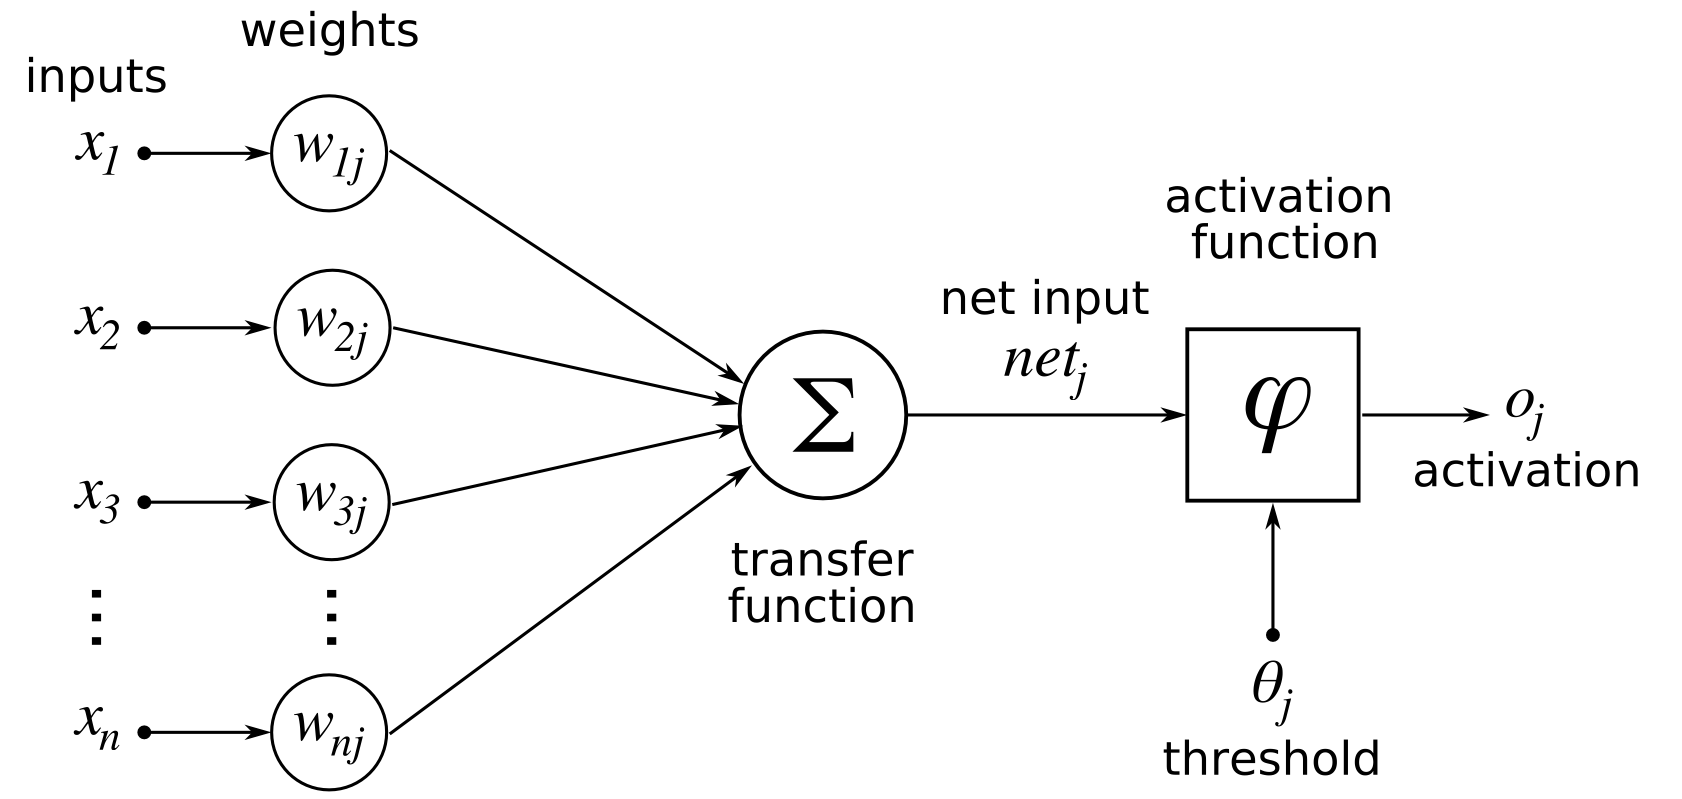
\includegraphics[width=.8\linewidth]{figures/ArtificialNeuronModel.png}
    \caption{Esempio di neurone artificiale \cite{wiki:xxx}}
    \label{fig:AN}
\end{figure}

A sua volta una rete neurale è composta da vari strati:
\begin{itemize}
    \item \textbf{Input Layer}: il primo strato della rete neurale
    e quello che riceve l'input esterno. Poiché la rete neurale
    è un modello matematico, l'input dovrà essere
    un vettore numerico. Questo vale anche se l'input da esaminare
    è una stringa di caratteri, come nel nostro caso.
    \item \textbf{Hidden Layer}: questo è lo strato intermedio della rete neurale in cui avviene
    il processo di apprendimento.
    Questo strato elabora gli input ricevuti dallo strato precedente
    modificando i pesi. Si possono avere anche più hidden layers
    \item \textbf{Output Layer}: Questo è l'ultimo strato della rete neurale.
    Fornisce i risultati finali ottenuti dalla rete neurale. Questo strato
    può essere composto anche da un solo neurone che fornisce
    un output binario (0 o 1) come sarà nel nostro caso(DGA o non DGA)
\end{itemize}

\begin{figure}[H]
    \centering
    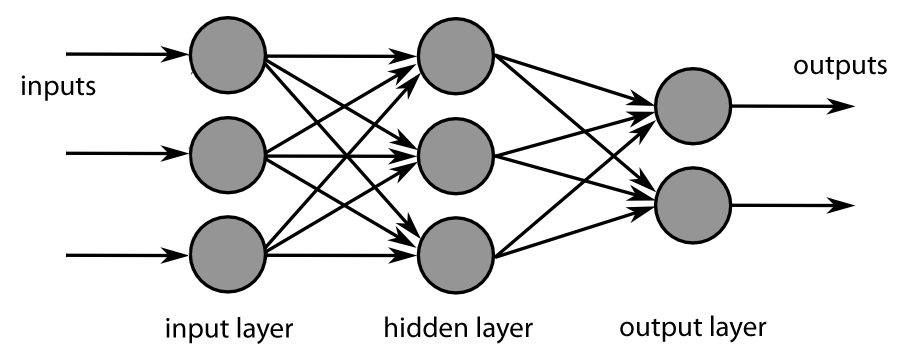
\includegraphics[width=.8\linewidth]{figures/MultiLayerNeuralNetwork.png}
    \caption{Esempio di rete neurale \cite{wiki:001}}
    \label{fig:ANN}
\end{figure}

Abbiamo inoltre vari tipi di reti neurali:
\begin{itemize}
    \item \textbf{Reti Neurali Feedforward}: Una rete Feedforward
    elabora le informazioni in un solo verso. Non ha né cicli
    né memoria delle informazioni passate. Questo tipo di rete
    è usato principalmente per riconoscimento di pattern o classificazioni
    \item \textbf{Reti Neurali Ricorrenti (RNN)}:
    A differenza di una rete Feedforward, in una RNN 
    i neuroni possono andare anche a formare dei cicli. 
    Questo permette alla rete di avere una specie di memoria
    e quindi di ricordare le informazioni passate. Usata
    per esempio per traduzione automatica o riconoscimento vocale.
    \item \textbf{Reti Neurali Convoluzionali (CNN)}: Questo tipo di rete
    è usato principalmente per dati strutturati a griglia ad esempio le immagini.
    Il nome "Convoluzionali" deriva dal fatto che la
    rete usa un'operazione matematica chiamata proprio
    convoluzione. Le CNN sono usate soprattuto nell'ambito della
    visione artificiale per il riconoscimento di oggetti
    \cite{Goodfellow-et-al-2016}.
\end{itemize}

\subsection{Sviluppo di una rete neurale}
Il primo passo per sviluppare una rete neurale è quello di
raccogliere i dati in un dataset. Nel nostro caso, dovendo riconoscere se un dominio
è lecito o \acrshort{DGA}, il dataset conterrà
entrambi i tipi di domini che potranno avere un etichetta, DGA o legit nel nostro caso, o no. Questi come detto in precedenza,
dovranno essere convertiti in un vettore numerico. A seconda di come
è strutturato il dataset possiamo avere vari tipi di allenamento:

\begin{itemize}
    \item \textbf{Supervised Learning}: È la tecnica più comune
    per allenare le reti neurali \cite{ayodele2010types}. In questo tipo di apprendimento,
    il modello viene addestrato su un dataset etichettato.
    \item \textbf{Unsupervised Learning}: In questo tipo di apprendimento,
    il modello, deve scoprire dei pattern o delle relazioni
    senza avere nessuna etichetta. Il modello deve trovare
    degli oggetti che condividono delle caratteristiche simili, chiamati
    cluster
    \item \textbf{Reinforcement Learning}: In questo tipo di apprendimento,
    ogni azione ha un effetto nell'ambiente che può essere positivo
    o negativo.
\end{itemize}

\noindent Si è soliti dividere il dataset in tre parti ovvero training set, validation set e test set.
Il \textbf{training set} è il dataset su cui viene addestrato
il modello, il \textbf{validation set} è una parte del training set
utile per riconoscere se il modello è in grado di generalizzare
su dati nuovi ovvero non va in overfitting o underfitting.
il \textbf{test set}, invece, è il dataset
su cui viene testata la precisione del modello.
Per la divisione del dataset non esiste una regola fissa,
ma solitamente il training set è più grande del validation set
e del test set. Un esempio potrebbe essere 70\% training set, 15\% validation set
e 15\% test set.
Successivamente viene deciso il tipo di rete 
neurale da usare, il numero di layers e il numero
di neuroni per ognuno di essi. Una rete troppo semplice
potrebbe non essere in grado di apprendere i pattern
nei dati (\textbf{Underfitting}), mentre al contrario,
una rete troppo complessa potrebbe imparare
troppo bene di dati e non generalizzare su dati nuovi
(\textbf{Overfitting}). Come detto in precedenza, il validation
set ci aiuta a capire se il modello va in overfitting o underfitting.
Successivamente vengono inizializzati i pesi di ogni neurone.
Questi possono essere inizializzati in modo casuale
o con altre tecniche più avanzate ad esempio
la \textbf{He Initialization} \cite{he2015delving}
(opzione di default quando si inizializza 
con attivazione ReLU).
Dopo di che si passa alla fase vera e propria di addestramento.
Il modello viene iterato per un certo numero di epoche su un batch di dati.
Un \textbf{batch} è un sottoinsieme del training set dopo il quale il modello
aggiorna i propri pesi. Ad esempio abbiamo un training set di 10000 dati
e un batch size di 100. Ogni 100 dati il modello calcolerà
l'output e la loss function, cioè la funzione che calcola
la differenza tra l'output previsto e quello reale,
e aggiornerà i pesi.
Il numero di epoche è un iperparametro che indica quante volte
l'algoritmo di apprendimento deve passare attraverso il dataset di training\cite{brownlee2018difference}.
Infine viene testato il modello sul test set e, se la precisione
è soddisfacente, il modello potrà essere usato.
\begin{figure}[H]
    \centering
    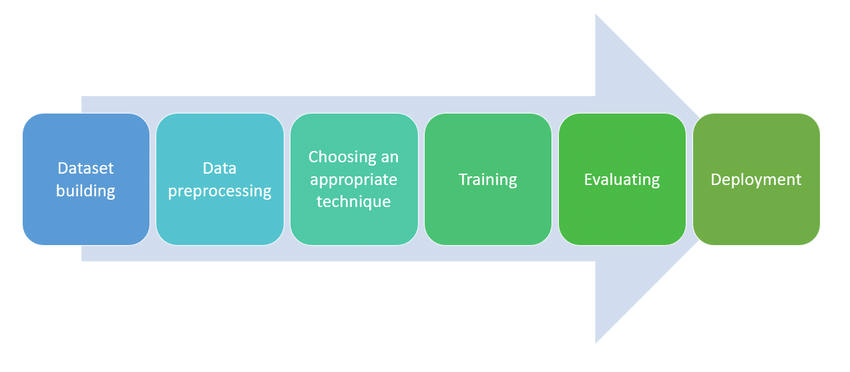
\includegraphics[width=.8\linewidth]{figures/Machine-learning-pipeline.png}
    \caption{Pipeline di un modello di Machine Learning \cite{phdthesishamza}}
    \label{fig:ML pipeline}
\end{figure}

\section{Algoritmi di Machine Learning adatti per DGA}

Ora che abbiamo visto i concetti di base del Machine Learning, delle reti neurali
e dei \acrshort{DGA}, vediamo alcuni degli algoritmi che possono essere usati
per rilevare i domini generati da \acrshort{DGA}.

\subsection{Random Forest}

Random Forest è un algoritmo esamble (cioè unisce più modelli) di Machine Learning supervisionato che usa un insieme di alberi decisionali
per classificare i dati. Un albero decisionale è un modello che usa appunto una struttura ad albero
per prendere decisioni. Un esempio può essere quello nella \cref{fig:decision tree}, in cui, a seconda di determinate
caratteristiche, l'albero decide se una persona rischia di avere un attacco cardiaco o meno.
Il problema principale del singolo albero decisionale è che è molto suscettibile
all'overfitting.
\begin{figure}[H]
    \centering
    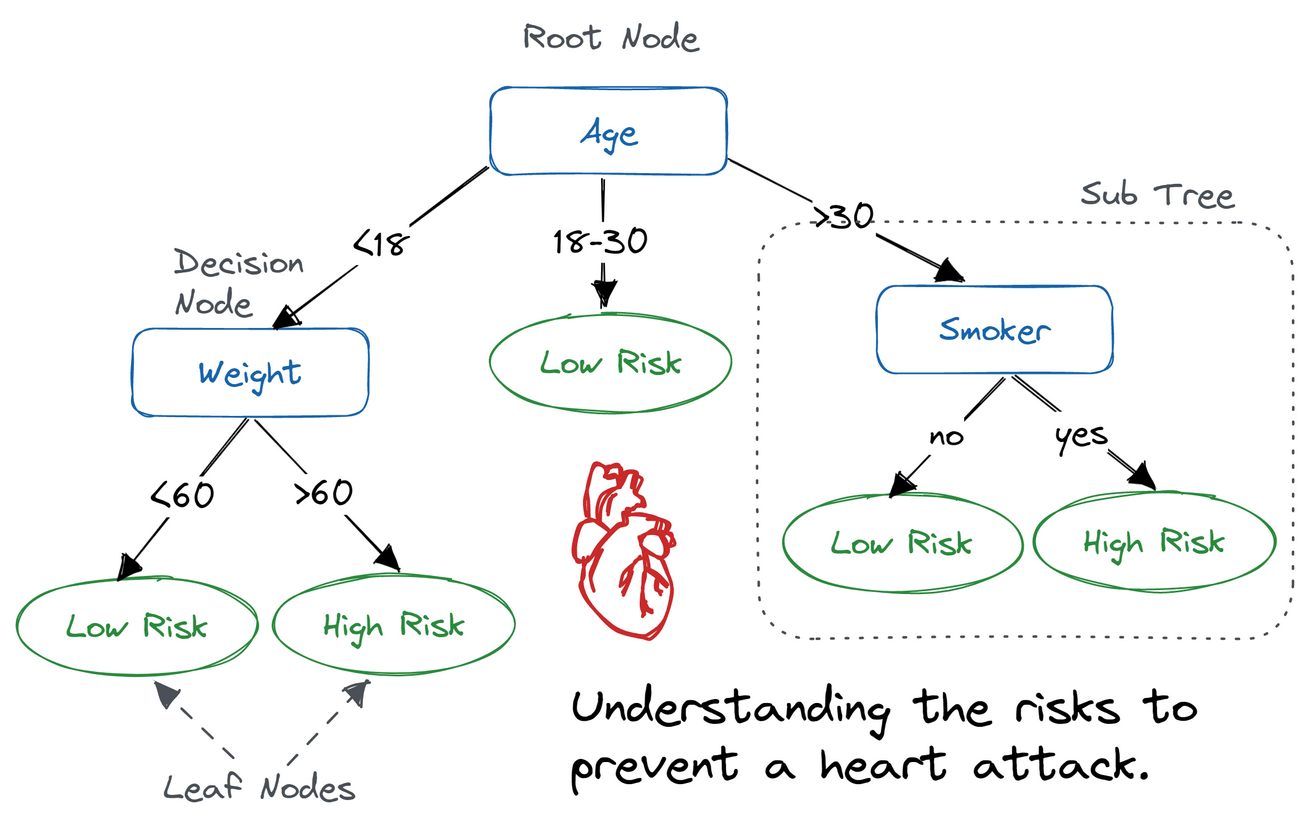
\includegraphics[width=.8\linewidth]{figures/Decision_tree_for_heart_attack.png}
    \caption{Esempio di albero decisionale \cite{decision_tree_image}}
    \label{fig:decision tree}
\end{figure}

\noindent Il random forest risolve questo problema aumentando 
l'accuratezza del modello sia in fase di training che in fase di testing. \cite{598994}
Random Forest usa un apporccio basato su feature, ovvero vengono selezionate
delle caratteristiche del dataset che possono essere utili per la classificazione.
Ad esempio, nel nostro caso, le caratteristiche potrebbero essere
il numero di vocali, lunghezza del dominio o l'entropia.
L'algoritmo funziona nel seguente modo:
Per prima cosa vengono creati $n$ alberi decisionali, ognuno
contenente una parte casuale del training set. Inoltre
ogni albero decisionale viene addestrato su un sottoinsieme casuale
di feature. Dopo di che, ogni albero fa la sua previsione,
e la previsione viene fatta in base a ciò che la maggior parte
degli alberi ha previsto se si tratta di un problema di classificazione mentre, qualora si trattasse di un problema di regressione,
la previsione finale sarà la media delle previsioni di tutti gli alberi.
L'algoritmo risulta tra i più usati per la sua semplicità e velocità
e per la sua capacità di gestire grandi quantità di dati e feature senza
perdere accuretezza.

\begin{figure}
    \centering
    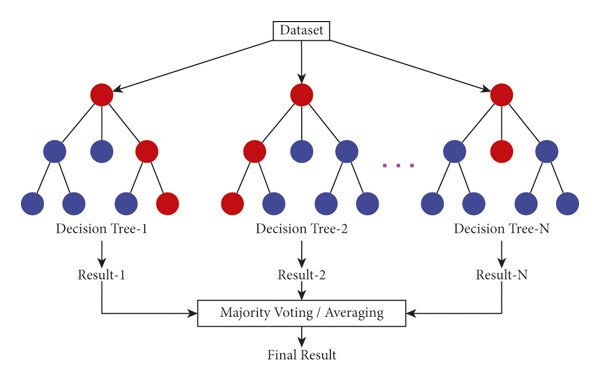
\includegraphics[width=.8\linewidth]{figures/Illustration-of-random-forest-trees.jpg}
    \caption{Esempio di Random Forest \cite{RFIMAGE}}
    \label{fig:random forest}
\end{figure}



% \subsection{XGBoost}
% XGBoost è un algoritmo di Machine Learning supervisionato

\subsection{Long Short Term Memory (LSTM)}

Le LSTM sono un tipo di rete neurale ricorrente (RNN). 
A differenza delle RNN tradizionali, esse sono in grado di
memorizzare informazioni per periodi di tempo più lunghi e possono
avere più strati nascosti. Create da Hochreiter e Schmidhuber nel 1997 \cite{LSTM1997},
le LSTM risolvono uno dei problemi più importanti
delle RNN standard, il vanishing gradient problem. Questo
problema si verifica poiché durante la backpropagation, i gradienti
tendono appunto a svanire, rendendo difficile l'apprendimento
di relazioni a lungo termine. 
Per risolverlo, le LSTM introducono una struttura dati vettoriale
chiamata \textbf{Memory Cell}(o cella di memoria). Questa viene
viene aggiornata ad ogni step tramite le operazioni decise dai "gates" (o porte).
La struttura delle LSTM è composta nel seguente modo:
\begin{itemize}
    \item \textbf{Input Gate}: determina quali nuove informazioni
    devono essere aggiunte allo stato della cella. Usa una funzione
    sigmoide per decidere quali valori saranno aggiunti e una tanh
    per creare nuovi valori
    \item \textbf{Forget Gate}: gestisce quali informazioni
    devono essere dimenticate dallo stato della cella. Usa una funzione
    sigmoide per decidere quali informazioni saranno mantenute o dimenticate.
    Se il valore è 0 le informazioni saranno dimenticate mentre se è 1 saranno mantenute.
    \item \textbf{Output Gate}: decide come sarà il prossimo hidden state
    Gli input sono passati a una funzione sigmoide e la cella
    aggiornata viene passata a una tanh e moltiplicata con l'output della sigmoide
    per decidere quali informazioni saranno passate.
\end{itemize}

\noindent Oltre alle LSTM tradizionali abbiamo anche le \textbf{BLSTM} (Bidirectional LSTM) che sono
composte da due LSTM, che elaborano i dati in due direzioni diverse.
A differenza del Random Forest, le LSTM usano un approccio featureless e imparano
direttamente dai dati. Alcuni usi delle LSTM sono ad esempio
il riconoscimento vocale o la traduzione automatica.

\begin{figure}[H]
    \centering
    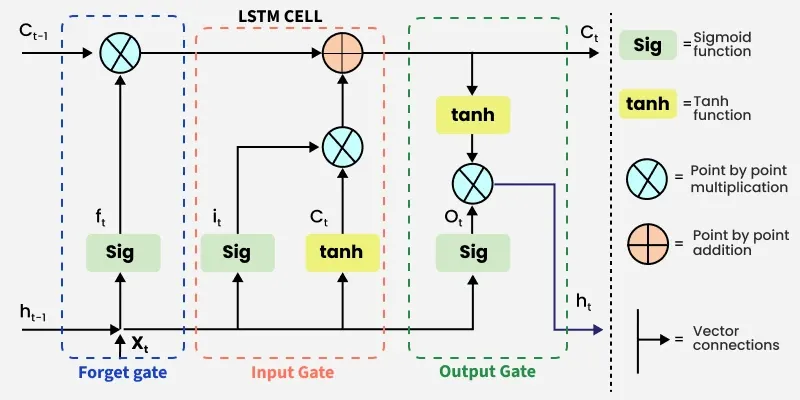
\includegraphics[width=.8\linewidth]{figures/gate_of_lstm.png}
    \caption{Struttura di un LSTM \cite{LSTM_image}}
    \label{fig:LSTM}
\end{figure}




\chapter{Progetto}
Il progetto ha come obiettivo quello di sviluppare un sistema
di rilevamento di domini generati da \acrshort{DGA} tramite
l'uso di tecniche di Machine Learning. 
Per il dataset ho deciso di usare il dataset di YangYang \cite{dataset_yangyang}
che contiene circa 1.5 milioni di domini \acrshort{DGA} e circa 1.5 milioni di domini legittimi.

\section{Linguaggi e librerie usate}
Per il progetto è stato usato il linguaggio Python poiché è il più usato
in ambito Machine Learning e analisi dei dati e offre una vasta gamma di librerie
adatte a questo scopo. Le librerie usate sono:
\begin{itemize}
    \item \textbf{Pandas}: libreria per la manipolazione e l'analisi dei dati.
    \item \textbf{Numpy}: libreria per il calcolo scientifico e l'elaborazione di array.
    \item \textbf{math}: libreria per le funzioni matematiche di base.
    \item \textbf{Scikit-learn}: libreria per il Machine Learning che offre vari algoritmi
    e strumenti per la valutazione dei modelli Nel nostro caso è stata usata per 
    la divisione del dataset in training, validation e test set,
    per l'implementazione del modello Random Forest e per il calcolo delle metriche di valutazione.
    \item \textbf{Tensorflow e Keras}: librerie per la creazione di reti neurali. Usate per la
    tokenization dei domini e per l'implementazione delle LSTM e BLSTM.
    \item \textbf{Matplotlib}: libreria per la visualizzazione dei dati e per la creazione di grafici.
\end{itemize}

\section{Metriche di valutazione}
Per valutare le prestazioni dei vari modelli si è deciso di usare i seguenti
parametri:
Accuracy, Pecision, Recall, F1-Score e Confusion Matrix. \hfill \break
Nel nostro modello un DGA ha come label 1(positivo) mentre un dominio legittimo ha come label 0 (negativo).
L'\textbf{Accuracy} è il rapporto del numero di predizioni
corrette sul numero totale di predizioni effettuate.
La formula è la seguente:
\begin{equation}
    Accuracy = \frac{TP + TN}{TP + TN + FP + FN}
\end{equation}

dove:
\begin{itemize}
    \item $TP$ è il numero di True Positive (Il numero di DGA classificati correttamente)
    \item $TN$ è il numero di True Negative (Il numero di domini legittimi classificati correttamente)
    \item $FP$ è il numero di False Positive (Il numero di domini legittimi classificati come DGA)
    \item $FN$ è il numero di False Negative (Il numero di DGA classificati come domini legittimi)
\end{itemize}

\noindent La \textbf{Precision} è il rapporto tra il numero di True Positive 
e il numero totale di predizioni positive effettuate.
La formula è la seguente:
\begin{equation}
    Precision = \frac{TP}{TP + FP}
\end{equation}
La \textbf{Recall} è il rapporto tra il numero di True Positive
e il numero totale di positivi ed è definita come segue:
\begin{equation}
    Recall = \frac{TP}{TP + FN}
\end{equation}
L'\textbf{F1-Score} è la media armonica tra Precision e Recall.
ed è definita come:
\begin{equation}
    F1-Score = 2 \cdot \frac{Precision \cdot Recall}{Precision + Recall}
\end{equation}
Nel progetto è stata usato Classification Report di scikit-learn
per calcolare queste metriche.
La \textbf{Confusion Matrix} è una matrice che mostra il numero di predizioni
corrette e sbagliate per ogni classe. Un vantaggio
della Confusion Matrix è che permette di vedere
quali classi sono state classificate correttamente e quali no e la quantità precisa di ogni classe.
\begin{figure}[H]
    \centering
    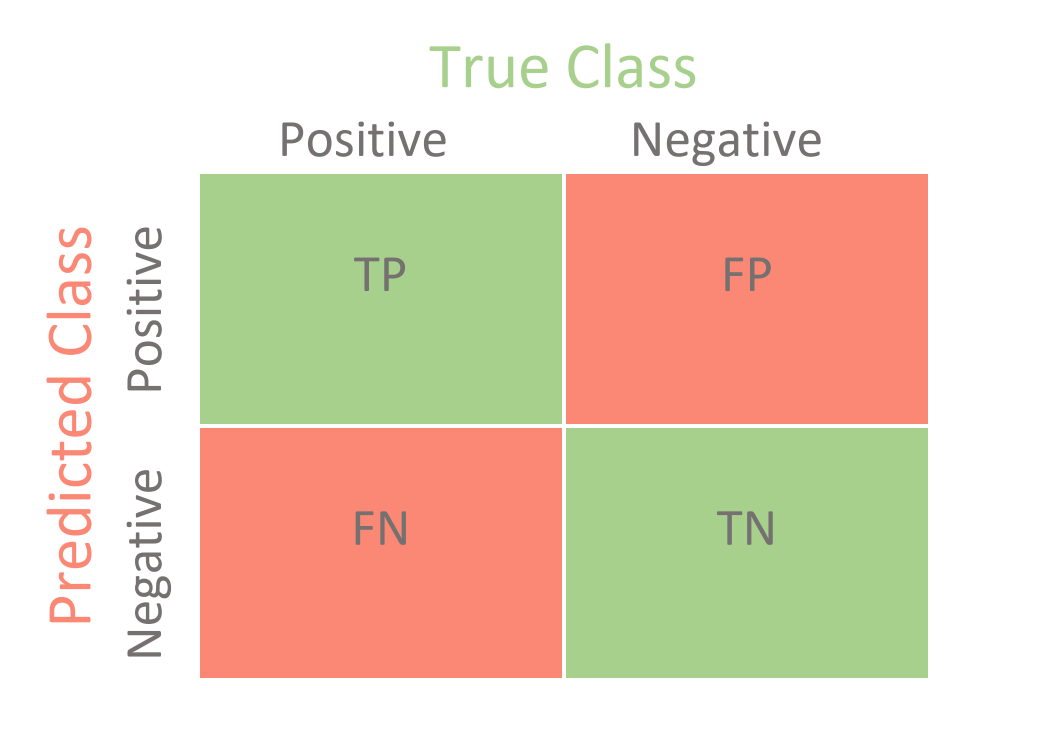
\includegraphics[width=0.6\linewidth]{figures/confusion-matrix.png}
    \caption{Esempio di Confusion Matrix \cite{confusion_matrix_image}}
    \label{fig:confusion matrix}
\end{figure}

\section{Test con Random Forest}

Il primo algoritmo testato è stato il Random Forest.
Qui non abbiamo bisogno di convertire i domini in
altri formati poiché il modello prenderà
come dati non il dominio in sé ma le sue caratteristiche(o features).
I parametri che prende il modello sono:
\begin{itemize}
    \item \textbf{n\_estimators}: il numero di alberi decisionali da creare
    Di default è 100. Si è provato ad aumentare il valore finchè, a parte un maggiore
    tempo di addestramento, non si è notato alcun miglioramento significativo.
    Alla fine si è deciso di usare il valore 200.
    \item \textbf{criterion}: la funzione usata per misurare la qualità di una divisione.
    Di default usa la funzione "gini".
    \item \textbf{max\_depth}: la profondità massima di ogni albero.
    Di default è None, ovvero gli alberi cresceranno fino a quando
    tutti i nodi saranno puri o fino a quando tutte le foglie
    conterranno meno di min\_samples\_split campioni.
    \item \textbf{min\_samples\_split}: il numero minimo di campioni richiesti
    per dividere un nodo interno. Di default è 2.
    \item \textbf{min\_samples\_leaf}: il numero minimo di campioni richiesti
    per essere una foglia. Di default è 1.
    \item \textbf{max\_features}: il numero massimo di feature da considerare
    per la divisione di un nodo. Di default è "sqrt" ovvero la radice quadrata
    del numero di feature.
    \item \textbf{random\_state}: il seed per la generazione casuale dei dati.
    Di default è None, ma facendo così il modello resituirà risultati diversi.
    Perciò si è deciso di dargli un seed fisso.
\end{itemize}
A parte per il random\_state e il numero di alberi gli altri parametri sono stati lasciati
con i valori di default poiché, dopo vari test non sono stati riscontrati grossi miglioramenti.
Inizialmente sono state usate come features la lunghezza del dominio, il numero di vocali,
il numero di consonanti, la quantità di numeri e l'entropia del dominio.
L'entropia misura la randomicità di una stringa e viene calcolata con la seguente formula:
\begin{equation}
    Entropy = -\sum_{i=1}^{n} p_i \cdot \log_2(p_i)
\end{equation}
dove $p_i$ è la probabilità di ogni carattere nel dominio. \hfil \break
Successivamente sono stati aggiunti altri parametri come il ratio tra consonanti e vocali,
il numero di trattini, l'entropia per bigramma, e il numero di consonanti e vocali consecutive.
Random Forest possiede un metodo che permette di calcolare l'importanza di ogni feature nel modello
chiamato \texttt{feature\_importances\_}
Grazie ad esso si è notato che le features più importanti sono state
l'entropia e quante vocali consecutive ci sono nel dominio.
Alcune features come se il dominio contiene un numero all'inizio o alla fine
o se il dominio contiene una wordlist di parole comuni ai DGA sono state
rimosse poiché non portavano un miglioramento significativo e anzi 
rischiavano di portare a un overfitting del modello.
\begin{figure}[H]
    \centering
    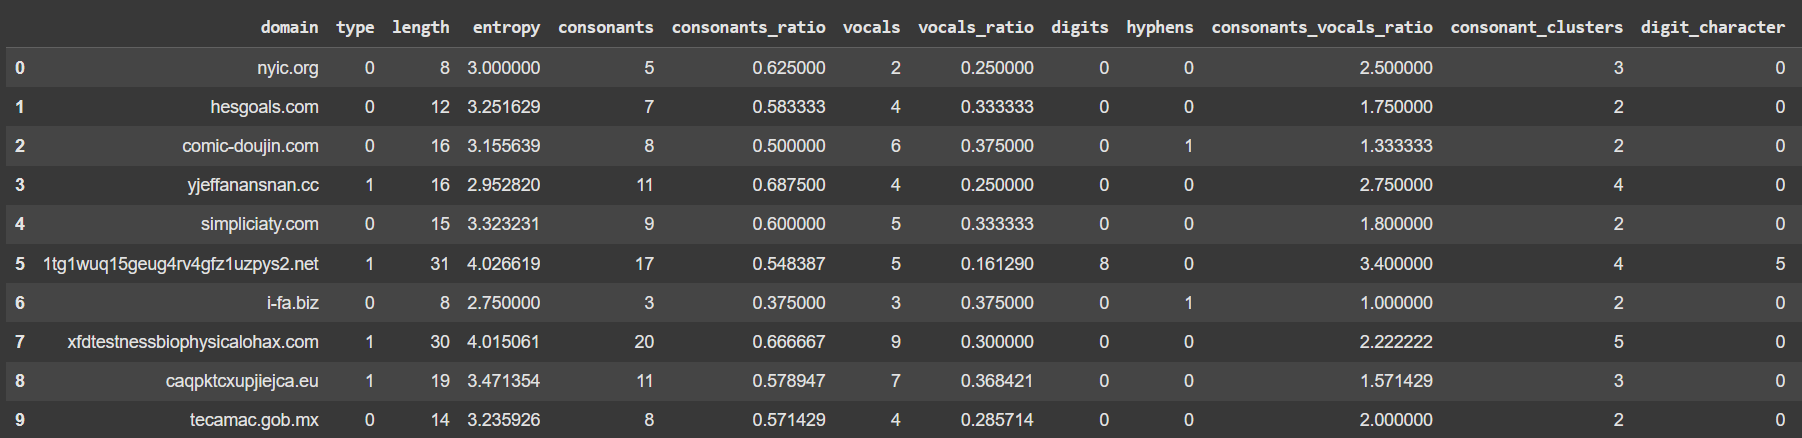
\includegraphics[width=.8\linewidth]{figures/RF_feature.png}
    \caption{Parte del dataset con i domini e loro features}
    \label{fig:RF feature}
\end{figure}
\noindent Dopo vari test si è raggiunta un accuratezza del 91\% ma
con risultati peggiori nel riconoscimento dei DGA come si può vedere nella \cref{fig:RF results}.

\begin{figure}[H]
    \centering
    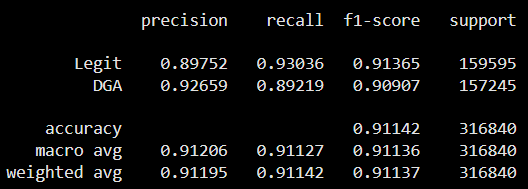
\includegraphics[width=.8\linewidth]{figures/RF_results.png}
    \caption{Risultati del modello Random Forest}
    \label{fig:RF results}
\end{figure}

\noindent Dalla Confusion Matrix \ref{fig:RF confusion matrix} si può vedere che il modello ha classificato
più di 5000 False Negative ovvero domini DGA classificati come legittimi rispetto ai False Positive.

\begin{figure}[H]
    \centering
    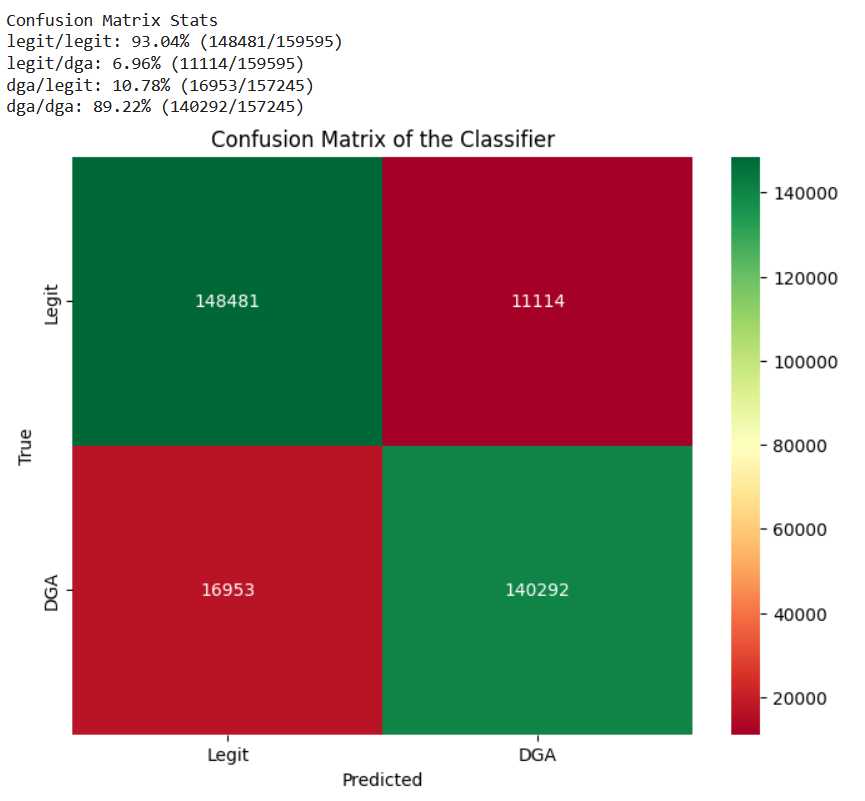
\includegraphics[width=.8\linewidth]{figures/RF_conf_matr.png}
    \caption{Confusion Matrix del modello Random Forest}
    \label{fig:RF confusion matrix}
\end{figure}




\section{Test con LSTM}
Poiché LSTM è un tipo di rete neurale adatto per il riconoscimento di pattern
ho deciso di usarlo per il progetto sia nella sua forma classica che in quella bidirezionale.
Il modello però non è in grado di leggere direttamente i domini.
Perciò bisogna convertire i domini in un formato leggibile dalla rete neurale e questo viene
svolto tramite un processo chiamato \textbf{Tokenization}.
Questo converte i dati in un formato leggibile dalla rete neurale.
Ci sono vari metodi di tokenization come word tokenization, che divide 
le stringhe in più parole o la character tokenization
che divide le stringhe in singoli caratteri. Essendo i domini delle semplici stringhe,
spesso senza parole di senso compiuto e con caratteri speciali come il punto o il trattino,
per questo progetto si è deciso di usare la character tokenization.
Per fare ciò si è usato il metodo \texttt{Tokenizer} di Keras.
Per questo modello si è deciso di usare
un modello sequenziale ovvero un modello in cui gli
strati sono disposti in sequenza uno dopo l'altro. \hfil \break
Il primo strato è uno strato di embedding che serve 
per convertire i caratteri in vettori numerici poiché
come detto in precedenza, le reti neurali
possono leggere solo numeri. \hfil \break
Successivamente nel modello è presente uno strato di LSTM
con 128 neuroni. Il numero di neuroni non 
è un valore fisso e non è determinato da una regola precisa.
Esso può essere scelto in base
alla complessità del problema o alla quantità di dati
presenti nel dataset. In generale con troppi neuroni si rischia di
andare in overfitting e con pochi il contrario. Dopo
vari tentativi, 128 neuroni è sembrata la scelta migliore poichè
con più neuroni il modello non imparava, rimanendo bloccato con un accuracy di 0.5 circa. \hfil \break
Dopo di che è stato aggiunto uno strato di dropout
ovvero uno strato che disabilita casualmente
un certo numero di neuroni durante l'addestramento 
per evitare l'overfitting. Anche il rate di dropout non
è un valore fisso.
Dopo è presente un altro strato LSTM come il primo e un dropout
e uno strato con attivazione relu con 64 neuroni che serve
a catturare pattern più complessi. Inizialmente
si era provato senza questo strato ma 
il modello aveva una precisione inferiore anche se di poco. Infine
l'ultimo è uno strato denso con attivazione sigmoide
che serve a classificare i dati in due classi, DGA e non DGA.
Per il training sono state scelte inizialmente 5 e poi 10 epoch.
Il modello però andava in overfitting, quindi si è deciso di aumentare
il numero di epoche a 50 e di usare l'early stopping, un metodo per interrompere
l'addestramento quando il modello non migliora più e per evitare l'overfitting. Alla
fine il modello l'addestramento si è fermato all'epoch 26 impiegando circa 30 minuti e poco più di 1 minuto per epoca.
Il modello raggiunge il 99\% di accuracy e un alto F1-Score nel riconoscimento di entrambi i tipi di domini,
come si può vedere nella \cref{fig:LSTM results}.

\begin{figure}[h]
    \centering
    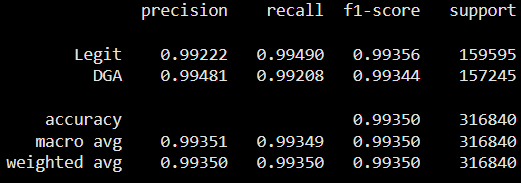
\includegraphics[width=.8\linewidth]{figures/LSTM_results.png}
    \caption{Risultati del modello LSTM}
    \label{fig:LSTM results}
\end{figure}

\noindent Dalla confusion matrix \ref{fig:LSTM confusion matrix} si può vedere che il modello ha classificato quasi tutti 
i domini correttamente. Leggermente di più sono i
False Negative ovvero domini DGA classificati come legittimi.
\begin{figure}[H]
    \centering
    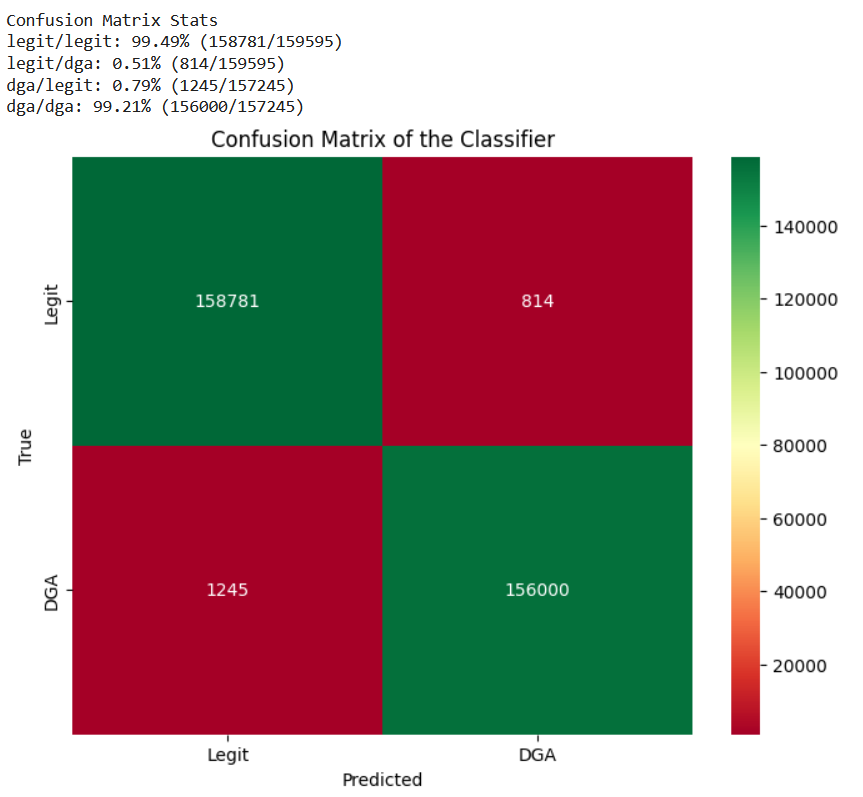
\includegraphics[width=.8\linewidth]{figures/LSTM conf_matr.png}
    \caption{Confusion Matrix del modello LSTM}
    \label{fig:LSTM confusion matrix}
\end{figure}

\section{Test con BLSTM}

Come detto in precedenza, le BLSTM sono una variante delle LSTM che
consentono di elaborare i dati in entrambe le direzioni.
Questo permette al modello di catturare meglio
i pattern nei dati.
Come nelle LSTM aumentare o dimunire il numero di neuroni
non ha avuto effetti positivi sul modello perciò si è deciso di usare anche qui
128 neuroni per ogni strato BLSTM e uno denso con attivazione relu con 64 neuroni.
Le tempistiche di addestramento, però, sono risultate
maggiori rispetto alle LSTM classiche, impiegando circa 4 minuti ad epoca e circa 1 ora e 10 minuti per 22 epochs totali.
I risultati sono stati molto simili a quelli delle LSTM come si può vedere nella \cref{fig:BLSTM results}.

\begin{figure}[H]
    \centering
    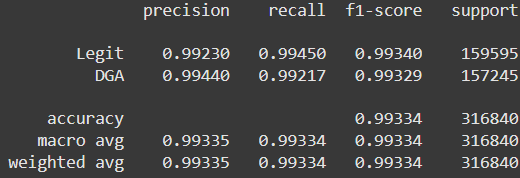
\includegraphics[width=.8\linewidth]{figures/BLSTM_results.png}
    \caption{Risultati del modello BLSTM}
    \label{fig:BLSTM results}
\end{figure}

\noindent Per quanto riguarda la confusion matrix \ref{fig:BLSTM confusion matrix}, il modello ha classificato
quasi tutti i domini correttamente. Il modello risulta più preciso anche se di poco rispetto alle LSTM classiche.
La maggior parte degli errori sono False Negative anche qui
\begin{figure}[H]
    \centering
    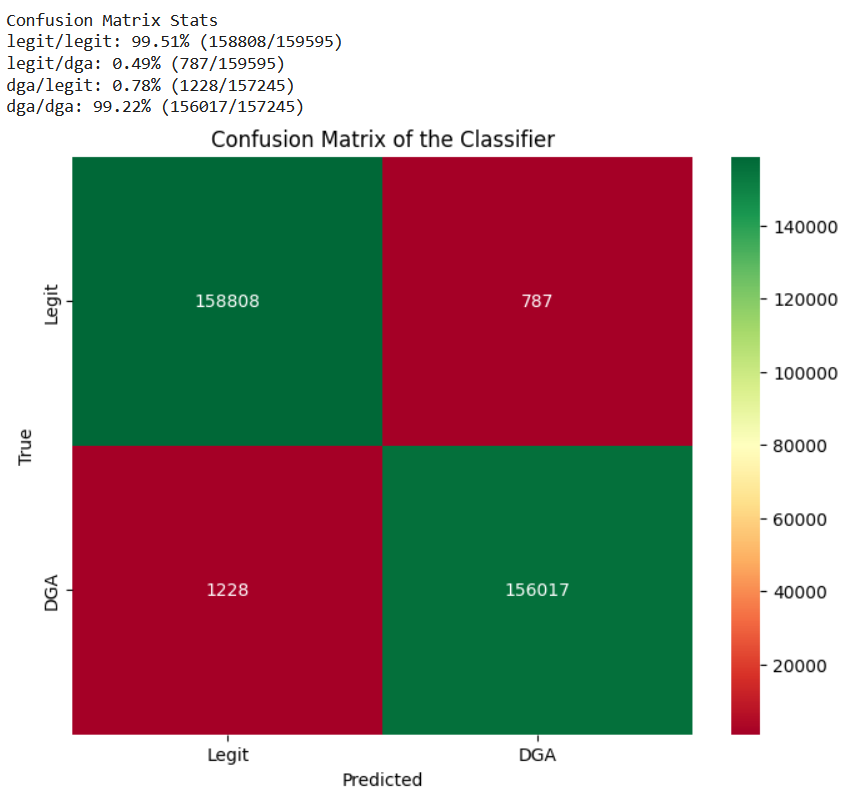
\includegraphics[width=.8\linewidth]{figures/BLSTM conf_matr.png}
    \caption{Confusion Matrix del modello BLSTM}
    \label{fig:BLSTM confusion matrix}
\end{figure}




% \chapter{Contribution}

% You may also put some code snippet (which is NOT float by default), eg: \cref{lst:random-code}.

% \lstinputlisting[float,language=Java,label={lst:random-code}]{listings/HelloWorld.java}

% \section{Fancy formulas here}


%----------------------------------------------------------------------------------------
% BIBLIOGRAPHY
%----------------------------------------------------------------------------------------

\backmatter

\bibliographystyle{IEEEtran} %prima era alpha
\bibliography{bibliography}

\begin{acknowledgements} % this is optional
 Optional. Max 1 page.
\end{acknowledgements}

\chapter*{Ringraziamenti}
\markboth{RINGRAZIAMENTI}{RINGRAZIAMENTI}
Con questo lavoro di tesi, si conclude il mio percorso di studi
sicuramente non facile ma che mi ha dato la possibilità di crescere sia
a livello personale che professionale.  \hfill \break
Ringrazio il mio relatore, il Prof. Mirko Viroli per essere stato sempre disponibile e avermi aiutato con il lavoro
e Lorenzo Magi e tutta Flashstart per l'aiuto dato e per avermi dato la possibilità di lavorare su questo progetto.  \hfill \break
Ringrazio la mia famiglia per avermi sempre supportato sia moralmente che economicamente. Senza
di loro non sarei mai riuscito a raggiungere questo traguardo.  \hfill \break
Ringrazio i miei amici in particolare l'associazione Sprite che hanno
reso questo percorso più divertente.
Ringrazio i bloccati e gli amici di Smash Bros per i momenti di divertimento e avermi dato un hobby per
staccare dallo studio.


\end{document}
